\documentclass[output=paper,colorlinks,citecolor=brown]{langscibook} 

\author{Samuel Awinkene Atintono \affiliation{Accra College of Education}}
\title{Lessons from the field: An Insight into the Documentation of 
 Gurenɛ Oral Genres
}  
\abstract{The paper discusses my eight months fieldwork experience of documenting endangered Gurenɛ (Mabia, Niger-Congo) oral genres which include riddles and folktales, sung folktales, songs and ritual performances between 2010 and 2012 in Bolga and Bongo in northern Ghana. It presents the documentary corpus of close to 100 hours of both audio and video recordings and discusses the strategies and challenges of documenting these genres. It is argued in this paper that though Gurenɛ with a speaker population of over 600 000 is not endangered, its oral genres such as riddles and folktales are vanishing and deserves attention to be documented. The paper draws attention of linguistic field workers and language documenters to pay attention to such languages and not to focus only on endangered or moribund languages. The documentation corpus from this project has been archived at the Endangered Languages Archive (ELAR) at SOAS, London. The lessons in this project can be used to document these genres in other Ghanaian or African languages for revitalization and preservation of these linguistic and cultural resources of language communities.}


\IfFileExists{../localcommands.tex}{
  \addbibresource{../localbibliography.bib}
  \usepackage{langsci-optional,langsci-branding}
\usepackage{langsci-gb4e}
% \usepackage{langsci-textipa}
% \usepackage{langsci-glyphs}
\usepackage[linguistics]{forest}
\usepackage{tabto}
\usepackage{multirow}
\usepackage{bbding}

\usepackage[normalem]{ulem}

\usepackage{tikz-qtree}

\usepackage{enumitem}

\usepackage{multicol}
\usepackage{stmaryrd} %double brackets

\makeatletter
\let\pgfmathModX=\pgfmathMod@
\usepackage{pgfplots,pgfplotstable}%
\let\pgfmathMod@=\pgfmathModX
\makeatother
\usepgfplotslibrary{colorbrewer}
\usetikzlibrary{fit}

\usepackage{jambox}
\usepackage{tikz-qtree-compat}
\usetikzlibrary{arrows, arrows.meta}
\usepackage{longtable}
\usepackage{subcaption}

  \makeatletter
\let\thetitle\@title
\let\theauthor\@author
\makeatother

\newcommand{\togglepaper}[1][0]{
%   \bibliography{../localbibliography}
  \papernote{\scriptsize\normalfont
    \theauthor.
    \thetitle.
    To appear in:
    Change Volume Editor \& in localcommands.tex
    Change volume title in localcommands.tex
    Berlin: Language Science Press. [preliminary page numbering]
  }
  \pagenumbering{roman}
  \setcounter{chapter}{#1}
  \addtocounter{chapter}{-1}
}

\newcommand{\bari}{\ipabar{\i}{.5ex}{1.1}{}{}}
\newcommand{\notipa}[1]{\textnormal{#1}}

\newcommand{\agre}{\textsc{agr}-\ol{eene}}

\renewcommand{\emph}[1]{\textit{#1}} % resetting a setting from ling-macros-modified (I think?)

% forest settings to make compact but (mostly) straight-spined trees:
\forestset{
fairly nice empty nodes/.style={
            delay={where content={}{shape=coordinate,for parent={
                  for children={anchor=north}}}{}}
, angled/.style={content/.expanded={$<$\forestov{content}$>$}}
}}

\forestset{sn edges/.style={for tree={parent anchor=south, child anchor=north}}}

\newcommand{\bex}{\begin{exe}}
\newcommand{\fex}{\end{exe}}

\newcommand{\bxl}{\begin{exe}}
\newcommand{\fxl}{\end{exe}}

\newcommand{\ix}[1]{\textsubscript{#1}}
\newcommand{\alert}[1]{\textbf{#1}}
\newcommand{\ol}[1]{\textit{#1}}


			\usetikzlibrary{shapes,arrows,positioning,decorations,decorations.pathmorphing,intersections}
\forestset{
nice empty nodes/.style={
    for tree={calign=fixed edge angles},
    delay={where content={}{shape=coordinate,for siblings={anchor=north}}{}}
},
}

\definecolor{dark-gray}{gray}{0.3}

%\usepackage{dingbat,pifont}


%%%%%%%%%%%%For arrows%%%%%%%%%%%%%

\newcommand\Tikzmark[2]{%
  \tikz[remember picture]\node[inner sep=0pt,outer sep=0pt] (#1) {#2};%
}
\NewDocumentCommand\DrawArrow{O{}mmmmO{3}}{
\tikz[remember picture,overlay]
  \draw[->,line width=0.8pt,shorten >= 2pt,shorten <= 2pt,#1]
    (#2) -- ++(0,-#6\ht\strutbox) coordinate (aux) -- node[#4] {#5} (#3|-aux) -- (#3);
}
\NewDocumentCommand\DrawDotted{O{}mmmmO{3}}{
\tikz[remember picture,overlay]
  \draw[->,line width=0.9pt,dotted,shorten >= 2pt,shorten <= 2pt,#1]
    (#2) -- ++(0,-#6\ht\strutbox) coordinate (aux) -- node[#4] {#5} (#3|-aux) -- (#3);
}
\NewDocumentCommand\DrawLine{O{}mmmmO{3}}{
\tikz[remember picture,overlay]
  \draw[line width=0.8pt,shorten >= 2pt,shorten <= 2pt,#1]
    (#2) -- ++(0,-#6\ht\strutbox) coordinate (aux) -- node[#4] {#5} (#3|-aux) -- (#3);
}
%%%%%%%%%%%%%%%%%%%%%%%%%%%%%%%%%%%%%


\newcommand{\baru}{ʉ}
\newcommand{\baruH}{\'\baru}
\newcommand{\baruL}{\`\baru}

\newcommand{\ep}{ε}
\newcommand{\epH}{\'\ep}
\newcommand{\epL}{\`\ep}

\newcommand{\schwa}{ə}
\newcommand{\schwaH}{\'ə}
\newcommand{\schwaL}{\`ə}

\newcommand{\oo}{ɔ}
\newcommand{\ooH}{\'\oo}
\newcommand{\ooL}{\`\oo}

\newcommand{\ds}{\textsuperscript{
	\hspace*{-2pt}\begin{tikzpicture}
		\draw[-{>[scale=0.5]}] (0,0.4) --(0,0.25);
	\end{tikzpicture}}}

\newcommand{\ch}{t͡ʃ}
\newcommand{\dz}{d͡ʒ}

\newcommand{\tgl}{ʔ}

%shortcuts for the complementizers
\newcommand{\mbuL}{mb\baruL}
\newcommand{\mbuHL}{mb\baruH\baruL}
\newcommand{\mbuLH}{mb\baruL\baruH}
\newcommand{\la}{lá}
\newcommand{\nda}{ndà}

\newcommand{\tsc}[1]{\textsc{#1}}
\renewcommand{\textscb}{ʙ}
\newcommand{\ipa}[1]{#1} %disable IPA

\newcommand{\SM}[1]{#1}

\DeclareNewSectionCommand
  [
    counterwithin = chapter,
    afterskip = 2.3ex plus .2ex,
    beforeskip = -3.5ex plus -1ex minus -.2ex,
    indent = 0pt,
    font = \usekomafont{section},
    level = 1,
    tocindent = 1.5em,
    toclevel = 1,
    tocnumwidth = 2.3em,
    tocstyle = section,
    style = section
  ]
  {appendixsection}

\renewcommand*\theappendixsection{\Alph{appendixsection}}
\renewcommand*{\appendixsectionformat}
              {\appendixname~\theappendixsection\autodot\enskip}
\renewcommand*{\appendixsectionmarkformat}
              {\appendixname~\theappendixsection\autodot\enskip}

\renewcommand{\lsChapterFooterSize}{\footnotesize}
 
  %% hyphenation points for line breaks
%% Normally, automatic hyphenation in LaTeX is very good
%% If a word is mis-hyphenated, add it to this file
%%
%% add information to TeX file before \begin{document} with:
%% %% hyphenation points for line breaks
%% Normally, automatic hyphenation in LaTeX is very good
%% If a word is mis-hyphenated, add it to this file
%%
%% add information to TeX file before \begin{document} with:
%% %% hyphenation points for line breaks
%% Normally, automatic hyphenation in LaTeX is very good
%% If a word is mis-hyphenated, add it to this file
%%
%% add information to TeX file before \begin{document} with:
%% \include{localhyphenation}
\hyphenation{
affri-ca-te
affri-ca-tes 
Līk-pāk-páln
pro-sod-ic
phe-nom-e-non
Chi-che-wa
Lu-bu-ku-su
Ngbu-gu
Boyel-dieu
Mat-chi
pho-neme
Mil-em-be
Nyan-chera
Mc-Pher-son
Tsoo-tso
Sku-pin
dis-tin-guishes
con-ser-va-tion
Me-dum-ba
}

\hyphenation{
affri-ca-te
affri-ca-tes 
Līk-pāk-páln
pro-sod-ic
phe-nom-e-non
Chi-che-wa
Lu-bu-ku-su
Ngbu-gu
Boyel-dieu
Mat-chi
pho-neme
Mil-em-be
Nyan-chera
Mc-Pher-son
Tsoo-tso
Sku-pin
dis-tin-guishes
con-ser-va-tion
Me-dum-ba
}

\hyphenation{
affri-ca-te
affri-ca-tes 
Līk-pāk-páln
pro-sod-ic
phe-nom-e-non
Chi-che-wa
Lu-bu-ku-su
Ngbu-gu
Boyel-dieu
Mat-chi
pho-neme
Mil-em-be
Nyan-chera
Mc-Pher-son
Tsoo-tso
Sku-pin
dis-tin-guishes
con-ser-va-tion
Me-dum-ba
}
 
  \togglepaper[23]%%chapternumber
}{}


\shorttitlerunninghead{Lessons from the field:  An insight into the documentation of 
 Gurenɛ genres}
\begin{document}
\shorttitlerunninghead{Lessons from the field:  An insight into the documentation of 
 Gurenɛ genres}
\maketitle

\section{Introduction} 
The paper provides some insights into the documentation of Gurenɛ oral genres based on eight months’ fieldwork that I have undertaken between 2010 and 2012 in Bolga and Bongo in northern Ghana, West Africa. The corpus includes riddles and folktales, sung folktales, songs, daily traditional court trials and ritual performances. 

A key contribution of the paper is the proposal to fieldworkers and language documenters not to focus only on documenting endangered and moribund languages but to pay attention to aspects of endangered linguistic resources of languages that are not classified as endangered. Ignoring these languages in our documentation agenda is a sure way to gradually lose some critical aspects of their cultural and linguistic resources of the speakers.

The paper also highlights some of the strategies used to document the Gurenɛ oral genres and the different types of genres documented. The corresponding number of hours of the recording of each genre is also provided. This is the first major documentation of this kind in the language. It provides a means for the revitalization and preservation of the linguistic and cultural resources of the language. Of late, some of the speakers especially the elderly and those living outside the homeland are engaged in various activities including the use of the social media (e.g whatsapp), music, youtube, the internet, churches, ethnic associations (e.g, BONABOTO, Terabuuriyele)   as a means to preserve the language and present it beyond its immediate borders.

One goal of the documentation was to collect the disappearing oral genres especially the riddles and folktales, sung folktales, songs performed by women and other oral genres as many as possible. These genres are fast disappearing in the communities as a result of the massive impact of modern life, motivated by the desire to adopt western values and commodities. Since there are no records of these genres or opportunity for the younger generation to learn them, I saw this as an opportunity to document and archive them. Related to this goal was also to make available the audio and video recordings to the community radio stations and members to take advantage of the digital technology and learn them. 

Another goal as is the case with many other documentation projects (cf. \cite{TrilsbeekWittenburg2006, Austin2003, Austin2006, Himmelmann1998, HimmelmannEtAl2006} is to ensure that the materials documented from the project are transcribed, annotated with metadata and deposited in a modern digital archive (e.g. ELAR) to provide a lasting record to prevent the loss of the genres. 

The paper is organised as follows; §2 provides the language profile with section §3 on the case for the documentation of endangered genres. §4 discusses the fieldwork setting and the activities while §5 focuses on the documentary corpus involving the audio and video recordings with §6 providing a discussion on the strategies used in documenting the folktales. In §7, the challenges on the field are presented and §8 concludes the paper. 

\section{Language profile}
Gurenɛ is classified as Mabia (Gur) and belongs to the Niger Congo languages in Africa. It is spoken in northern Ghana, West Africa. It is sub-classified as a northwestern Mabia language with its closest relative being Dagaare and Moore spoken in Burkina Faso \citep{Naden1989, Bendor-SamuelHartell1989, Bodomo1994, Bodomo2004, Bodomo2020}.  2000,  It has about 600,000 speakers based on the Ghana Statistical Service Census Report (2010). This figure obviously is not accurate since the census did not take into account the language that the people speak but their ethnic membership. Of course, most of the ethnic members do speak the language and transmit it to their children. However, the problem with the ethnic membership criterion is that there is lack of clarity in the label. For example, in the 2010 Census, an old ethnic label Mole-Dagbani was used to refer to all the over twenty different linguistic groupings in northern Ghana of which Gurenɛ speakers are part. This label was used especially in cases where the speakers migrated to other communities in southern Ghana. So, people identified to belong to the Gurenɛ ethnic group were those in the homeland during the census. This has led to a misrepresentation of the actual number of speakers of the language and hence my reason for the mistrust of the figure.

Further, there is also the tendency for smaller ethnic groups within to identify themselves with their inner group for socio-political reasons and therefore missed being counted. For example, speakers from Bolga west, though are Gurenɛ speakers will usually identify themselves as belonging to Kasina-Nankani ethnic group (the speak Kasim or Nankani) and indeed were not counted as speakers although they belong to this language group. 

Today, there is evidence from my recent fieldwork \citep{Atintono2013, Atintono2020}, and Bodomo's \citeyear{Bodomo2004, Bodomo2020} fieldwork to suggest that the number of speakers could be as high as 800,000. Other anecdotal evidence comes from the community based on district health census and livelihood intervention programmes data which support our estimate and suggest that the figure is higher than reported. 

Gurenɛ is one of the five dialects of Farefari besides Boone, Nabt, Nankani and Taln \citep{Dakubu1995, Nsoh1997, Nsoh2011, Atintono2002, Atintono2004, Atintono2011, Atintono2013, Atintono2019}. All the five dialects are mutually intelligible. It is important to point out that in the language classification literature there have been a misrepresentation of the language name leading to spellings such as Frafra, Gurenne, Gurune and Gureni. Farefari is a cover term representing all the five dialects. However, Gurenɛ is privilege to have a unified orthography as far back in 2001. Thus, Gurenɛ has been standardized and today has been considered as a language as a result of its current status of been codified. My position has been that it is a standard dialect of Farefari as shown in my previous works \citep{Atintono2002, Atintono2004, Atintono2011, Atintono2013}. This is not new in linguistics as standard dialects emerged as languages due to their prestige status of been used in writing.

The language is also studied in the Universities (e.g, University of Education, Winneba) and the Colleges of Education in Ghana but it is yet to be introduced at the early grade, primary, and secondary school levels as a subject of study. The College of Languages Education, Ajumako at the University of Education, Winneba is one main institutions in Ghana that trains both undergraduates and postgraduates in Gurenɛ. The present documentation project focused on Gurenɛ and the Boone dialects as spoken in Bolga and Bongo.

\section{The case for documenting vanishing genres in non-endangered languages }
Recent interests in language documentation and description by linguistic fieldworkers is as a result of global concerns about language threat, endangerment and death \citep{HaleEtAl1992, Himmelmann1998, HimmelmannEtAl2006, GrenobleWhaley1996, Crystal2000, Crystal2003, Woodbury2003, Austin2003, Austin2006, GippertEtAl2006, Bowern2015, ChelliahWillem2010, EssegbeyEtAl2015}. Consequently, a great deal of attention has been paid to language endangerment and documentation issues in the last few decades. Despite these efforts, there has not been a balance in actual practice in terms of the languages that have been documented across the continents and funding support for language documentation projects as far as the literature show. 

The attention of fieldworkers and funding for documentation projects from organizations such as UNESCO, NSF, DOBES, ELDP so far are skewed towards documenting endangered languages in Australia and the Americas with a few on African languages (cf. \citealt{EssegbeyEtAl2015}).  There is also a huge support for documentation projects that tend to focus on severely endangered or moribund languages. In this respect, a critical defining criterion is that languages with fewer speakers of about 1 to 100 who are older speakers but without younger speakers stand a good chance for support for documentation from endangered languages documentation funding agencies. 

The reality, however, is that there are many languages in Africa with large numbers of speakers from a few thousand to hundreds of thousands with many aspects of their linguistic resources endangered. Such languages do not fit in the documentation agenda and are usually left out. The argument that is pushed in the language documentation discourse is that such languages fit into the language preservation and revitalization projects but not language endangerment projects. I take a different position and propose that equal attention should be paid to such languages and be treated as endangered so long as there is sufficient justification to point out that some aspects of their linguistic resources are vanishing or dying in these languages. 

Gurenɛ is one of such languages and cannot be classified as an endangered language with a speaker population of over 600,000 but with certain aspects of its linguistic and cultural resources such as riddles and folktales vanishing. 

To put the discussion in context, it is important to state the defining criteria for endangered languages.  A language is said to be endangered when it is at risk of disappearing within a generation or two with only elderly fluent speakers and no younger generation learning the language or are speakers \citet[4]{Thomason2015}. There are various degrees of language endangerment or vitality as depicted in the endangered languages literature. In particular, Moseley’s \citep{Moseley2012} UNESCO Atlas of the world’s languages in danger and \citegen[6]{UNESCO2011} discussion on degrees of language endangerment in a document titled “Language Vitality and Endangerment” outlined six stages which are stated below:

\todo[inline]{Please verify that you intend to cite \citet{UNESCO2011} instead of \citet{UNESCO2003}, which is where the factors and stages in question were first laid out. Also please check the page numbers.}

\begin{itemize}
\item A language is safe when there is intergenerational transmission and this is not interrupted.
\item 	It is said to be vunerable when the spearkers use the language in restricted or in certain discourse contexts such as home alone.
\item 	Definitely endangered when children no longer learn the language as mother tongue in the home.
\item 	A severely endangered language refers to a situation where the language is spoken by grand parents and older generations without transmission to younger generation and even rarely among themselves.
\item 	It is also critically endangered when the younger speakers are grand parents who speak the language less frequently.
\item 	Lastly a language is extinct or dead when there is no more any existing speaker. 
\end{itemize}
Some language documentation experts such as \citet{GrenobleWhaley1998} also define language endangerment similar to UNESCO scale but not necessarily identical to include; At risk, Disappearing, Moribund, Nearly extinct, and Extinct.

\todo[inline]{Please make sure that you intend to cite \cite{GrenobleWhaley1998}, the book, which was not in the original bibliography, and not \cite{GrenobleWhaley1996}, the IJSL paper that came two years prior. And, if so, please verify that this is the correct work from 1998}

On language vitality, \citet[5]{UNESCO2011} identified nine criteria which include intergenerational transmission, community member’s attitude towards their own language, shifts in domains of language use, governmental and institutional language attitudes and policies, including official status and use, type and quality of documentation, response to new domains and media, availability of materials for language education and literacy, proportion of speakers within the total population, and absolute number of speakers.

Based on these classifications of the stages of language endangerment, it is safe to conclude that Gurenɛ is not endangered because there is intergenerational transmission with both older and younger speakers. However, the language could be described as vulnerable because it is largely spoken at home and other social contexts such as market, daily interactions and at social events such as funerals, ethnic association meetings, and naming ceremonies.

In terms of vitality, out of the nine criteria, Gurenԑ will missed only one and that is no official status is accorded to the language by government especially to include the language in the school curriculum at the primary and secondary school levels. The people have sent many requests and petitions to the Ministry of Education to include the language in the official policy of the Ghanaian languages since 2002 but received no response.

Despite the fact that the language as a whole is not endangered, some aspects of its linguistic repertoires are critically endangered. They include riddles and folktales, sung folktales, songs, descriptive events and ritual performances. This is because these genres are no longer practised in the community for over three decades. Only a few elderly speakers (numbering about 5) in the community with the youngest been over 50 years and the oldest over 70 years by 2010 have knowledge in the narration of the riddles and folktales in particular. 

The various social contexts in which the folktales were narrated no longer exist. For example, they used to be narrated in the evening by grand parents with children sitting around the fire in the evening (around 7.00pm) after dinner in front of the traditional compound. This was a source of entertainment as well as a means of inculcating moral lessons to children through the messages conveyed in the folktales. These genres are classified as oral literature comparable to western written literature which are used for the teaching of; expressing of thought, history, collective wisdom, language and literature. 

The traditional home setting or context for the narration of these tales have been altered due to the adoption of western modes of entertainment. Thus, they have long since been replaced this traditional mode of entertainment with television sets and videos. This has further facilitated the endangerment and subsequent vanishing of the genres.

At the time of my documentation project between 2010 and 2011 as indicated in the preceding paragraph, only five (5) older men with ages between 50 and 70 years had expert knowledge in narrating the riddles and folktales. However, by February 2011 one of these five experts who mentored the other four experts had passed away. The contribution of the present work is the fact that but for this project, the community would have lost this genius narrator with his knowledge in this endangered genre. African oral genres such as riddles and folktales, sung folktales are far less familiar in western cultures and are less documented. 

The Gurenɛ community like most other African communities, however, have no records of these genres for the younger generation to learn and practise them. This lack of records partly motivated the documentation of these genres to provide a lasting record in an archive and also with a keen interest in revitalising them. 

The project also provided the opportunity for the recordings to be made available on CDs and DVDs for use by the community members and this is helping with the re-learning of these genres by the younger speakers. Quite recently, some of the riddles and folktales have also been shared on social media such as WhatsApp and YouTube for use by speakers and this is fast gaining grounds. The archived materials at the Endangered Languages (ELAR) is open access for most of the materials for both the community members and the research community. In Ghana, there are no well-established digital archives except a university’s online library resource depositories which are often not open resources. Nonetheless, I have made copies of the recordings available to the Department of Gur-Gonja Languages Education at the University of Education, Winneba, where Gurenԑ is taught.

It is for the reasons discussed in the preceding endangerment paragraphs on the genres that  
I am proposing in this paper that though the language documentation agenda focuses on the endangerment of the entire language, it is also important that we pay attention to languages that may appear not to be at risk and yet have some of its important aspects critically endangered like the Gurenɛ’s case. Indeed, the same can be argued for most of the Gur languages spoken in northern Ghana as they have large number of speakers with intergenerational transmission and yet have their oral genres disappearing (see \citealt{Bodomo2004, Bodomo2020}).

\section{The fieldwork setting and activities}
The fieldwork took place in six (6) communities in Bolga and Bongo between February 2010 and July 2011. The communities were typically rural except a few that were close to Bolga town such as Tanzui, Soe and Bukere where I recorded some of the folktales, funeral and ritual performances events. I spent eight (8) months on the field for the documentation. The first major field visit took place from February-June 2010. During this period, I recruited five documentation team members and one research assistant to assist in the recording on the field and transcription of the data. They were trained to acquire some basic skills to understand the project and the use of the audio and video recording equipment in language documentation. 

I also identified five (5) experts in folktale narration and two (2) groups of sung folktale narrators in the communities with the help of the community members. We arranged with these teams and did a lot of the audio and video recordings in their communities either at a school compound or at the home of the performer. The arrangement to have the folktales performed in these two contexts are staged events as the natural or normal context for the performance used to be in the evenings during occasions such as newly married couple homes, home of a family head or when an important guest for the community visited and was passing the night. The folktale performances were for entertainment.  

Together with my documentation team members, we had narrative sessions with each of the narrators at least once in a week for about six months even though some of the narrators frequently cancelled work appointments due to some emergencies. The communities were relatively far apart. Two of the narrators were from Soe and Bukere in Bolga while one narrator was from Yorogo (about 15km north of Bolga), and the most talented narrator who used to ply his trade in Bolga in the 1960s and 1980s had retired to his village at Kansuo (Namoo) of about 35km away from Bolga at the fringes of the Ghana and Burkina Faso border in the Bongo district. The sung folktale groups were both from Beo and Sapooro respectively located east of Bolga. 

While the folktale narrators had between two (2) to seven (5) members in a team that of the sung folktale groups had between seven (7) to twenty (20) members in a group.

Apart from the five expert narrators’ tales that we recorded, we came across by chance a blind narrator in Bongo who was identified by a community member. We had two recording sessions with him. Although, he had a good knowledge in folktales he did not have a team to support him like the other groups. He told us he learned the tales from his parents while growing up in the 1950s. He invited two of his friends to support him but they were not good respondents.

Other events that we recorded during the period include interviews with some elders on funeral performances and the rituals associated with burial. We also participated in chieftaincy installation events and traditional court proceedings at the Bongo palace. The paramount chief of Bongo (Naba Lem Yaarum) was very enthusiastic about our project and granted us interviews on the history of the Bongo chieftaincy and also the rituals associated with the installation processes. 

Recording of women’s songs was also another major activity that we under took on the field. We had a women’s group from Sumbrongo, a town located at about ten kilometers west of Bolga who agreed to perform for us. We had four recording sessions with them. While on the field we took advantage to document daily conversations and other cultural events that were spontaneous in the communities whenever community members drew our attention to them.

I also conducted elicitation sessions with other consultants to collect data specific on the grammar and semantics of positional verbs for the writing of my PhD thesis which was part of the award of the ELDP grant. 

The follow-up fieldwork was from May-June 2011. This last visit was mainly to cross-check gabs in the data with the consultants and do a few more elicitations and recordings of the folktales. The transcription of the recordings and the final preparation of the metadata constituted the main activities during this visit. It is important to point out that fieldworkers should ensure that the thin and thick metadata are properly recorded while they are on the field. But for the follow-up field trip, I had difficulty identifying names of some contributors, places the data was recorded and even dates and times. This is because we did not record some of the metadata information properly while we were on the field.

Unfortunately, on my second visit, the expert folktale narrator from Namoo (Azulemania) had died in February 2011. I had planned to meet him and record a few more tales and cross-check a few things with him but it was too late. The community members were, however, happy that my documentation record will help to preserve some of his folktales for future generations.


\section{The audio and video corpus}
The documentation project produced a large volume of both audio and video recordings of a variety of genres. These are shown in Table 1 and Table 2 below. Most of this corpus has been transcribed and annotated using ELAN and are archived with metadata at ELAR, SOAS in 2012 and can be accessed at    https://www.elar.soas.ac.uk. Though this is an open access you will need permission for identification purposes from the archivist to gain access.

\begin{table}
   	\begin{tabular}{p{2.5cm} p{2.5cm} p{1cm} p{2.5cm} p{2.5cm}  }
    \lsptoprule
       \textbf{Genre} & \textbf{Length of Recording} & \textbf{Genre Count }& \textbf{Transcription} & \textbf{Archived} \\
\midrule
Riddles & 1hr: 15 mins & 160 & 1 hr : 15 mins & 0hr:30 mins \\
Folktales & 25 hrs : 30 mins & 350 & 12 hrs: 15 mins & 10 hrs: 40 mins\\
Sung Folktales & 5hrs : 30mins  & 150 & 3 hrs : 30 mins & 2 hrs :30 mins \\
Women Songs
& 6hrs: 50mins 
& 75
& 3 hrs: 30 mins
& 2 hrs : 30 mins \\
Daily Conversations
& 4hrs: 20mins 
& 35
& 2 hrs:00mins
& 1hr:00min \\
Historical Narratives
& 5hrs: 45mins 
& 5
& 2 hrs: 30 mins
& 1hr : 30mins \\
Palace Genres
& 5hrs: 25mins 
& 25
& 3 hrs: 25 mins
& 2 hrs: 20 mins \\
Descriptive Text
& 1hr: 15mins 
& 5
& 1 hr: 15 mins
& 1 hr : 15mins \\
Burial and Funeral Genres
& 5hr: 40 
& 10
& 2 hrs: 10 mins
& 1 hr: 10 mins \\
Ritual Performances
& 2hr : 20 
& 15
& 1 hr: 15 mins
& 1 hr: 15 mins \\
\midrule
\textbf{Total}
& \textbf{63hrs:50mins}
& \textbf{830}
& \textbf{33hrs:05mins}
& \textbf{25hrs:00min} \\
\lspbottomrule
    \end{tabular}
    \caption{Audio recordings of the oral genres}
    \label{tab:audio}
\end{table}


 \begin{table}
 	    \begin{tabular}{p{2.5cm} p{2.5cm} p{1cm} p{2.5cm} p{2.5cm}  }
    \lsptoprule
     
       \textbf{Genre} & \textbf{Length of Recording} & \textbf{Genre Count }& \textbf{Transcription} & \textbf{Archived} \\
\midrule
    Riddles	& 0hr: 30mins 	& 75	& 0hr: 30mins	& 0hr: 30 mins  \\ 
Folktales	& 10hrs: 30mins 	& 200	& 5hrs: 0 mins	& 5 hrs: 0 mins \\
Sung Folktale	& 6hrs: 30mins 	& 150	& 3hrs: 30 mins	& 2 hrs :30 mins \\  
Women Songs	& 4hrs: 30mins 	& 50	& 2hrs: 30 mins	& 2 hrs: 30 mins \\
Daily Conversations	& 1hr: 20mins 	& 20	& 1hr:00min 	& 0hr:0 min  \\
Historical Narratives	& 0hr: 30mins 	& 20	& 0hr: 30 mins	& 0hr : 30mins \\
Palace Genres	& 4hrs: 30mins 	& 25	& 3hrs: 25 mins	& 1hr: 30 mins \\
War Dance	& 2hrs: 15mins 	& 5	& 0 hr: 0 mins	& 2hrs : 15mins \\
Burial and Funeral Genres	& 4hrs : 40mins 	& 10	& 2hrs: 10 mins	& 1hr: 10mins \\
Ritual Performances	& 0hr: 0min	& 0	& 0 hr: 0mins	& 0hr: 0 mins \\
Total
	& 35hrs:15mins
	& 555	&18hrs:35mins	 & 15hrs:55mins \\
    \lspbottomrule
 
    \end{tabular}
    \caption{Video recordings of the oral genres}
    \label{video}
 \end{table}
Notice that in Table 1 and Table 2 above, there is a difference between the audio and video recordings in terms of the length of recording. There are a number of factors that account for this. First, it is much easier to do audio recording on the field than video. Further, as you might have observed, some of the genres like ritual genres are not on video because we were never permitted to use video to record. 

Besides, the type of equipment you use to record will also contribute to how much data you can record.  In my case, I used a Panasonic video camcorder, which could only record, on mini cassettes with a maximum of one hour. So, there were instances where we ran out of cassettes to record. But the digital audio recorder used SD cards and could record for longer hours of between three to five hours depending on the capacity of the card.  This is the advantage of the audio recorder over the camcorder. Even if we had a camera that could record longer hours there was also the problem of the time of the day. Most of the recordings in the communities took place in  late afternoon (from 4.00pm on wards) running late into the night. Per the tradition, they were narrated when it is nightfall after dinner. Thus, when it is nightfall it becomes difficult to do video recording without sufficient light. Also, the fact that my team and I were operating in rural settings made it difficult to have lights.

Apart from the audio and video recordings, I have also taken about one thousand (1,000) still pictures out of which two hundred and twenty-five (225) photos have been archived. The pictures depict different scenes of the folktale narration sessions, sung folktale performances, women song performances, cultural events such as funerals and chieftaincy installation events in Bongo and the elicitation sessions. Figures 1 to 6 below present examples of the scenes of the folktale narration sessions and other events. The arrangement is typically a semi-circle or a circle with the narrator and his team at the front row (Figure 1 below) while the audience sit behind or in front with space at the centre where occasionally the audience or the narrators may step in the space to dance to a folktale song.

\begin{figure}
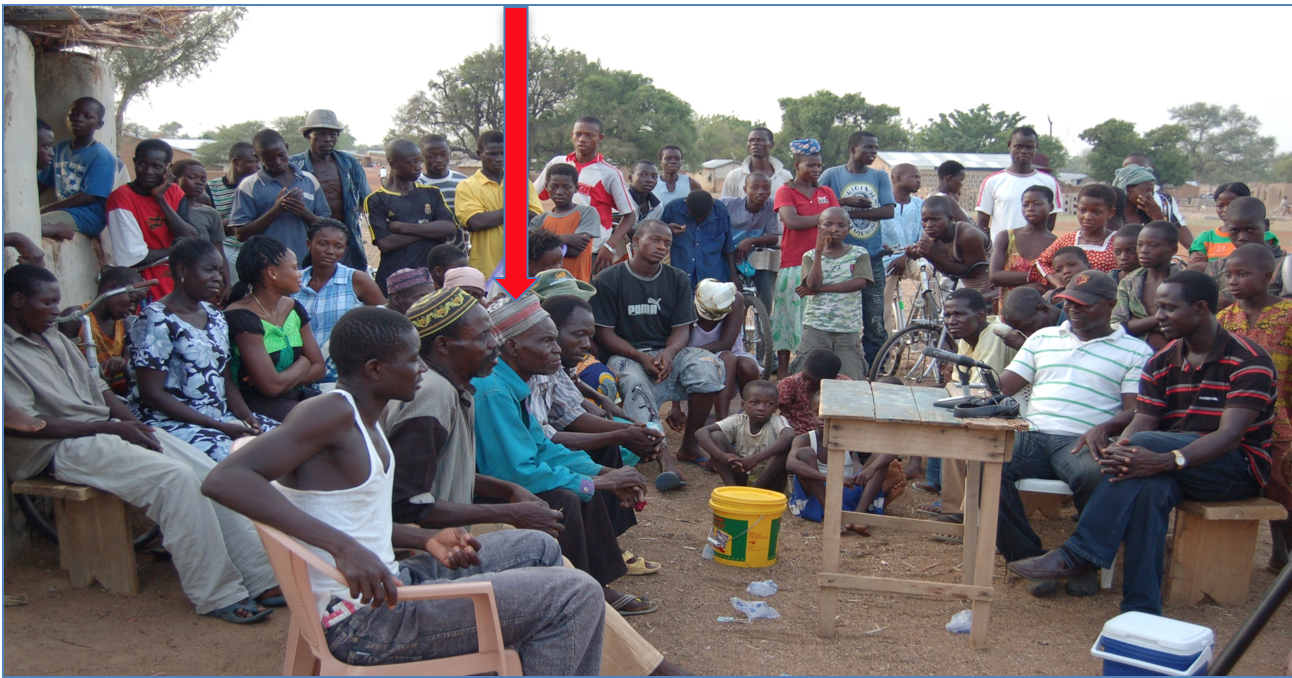
\includegraphics[scale=0.55]{../figures/azulemania.png}
\caption{: Folktale narration session at Kansuo (Namoo, Bongo) by Azulemania (seated 3rd from left first row 
 	 in light blue shirt, arrowed) with his team members. At the extreme right row (1st row) monitoring 
 	the recordings are Samuel Atintono (the documenter in red and black T-shirt) and James Akolgo 
 	(white and green T-shirt), May 2010.}

\end{figure}

\begin{figure}
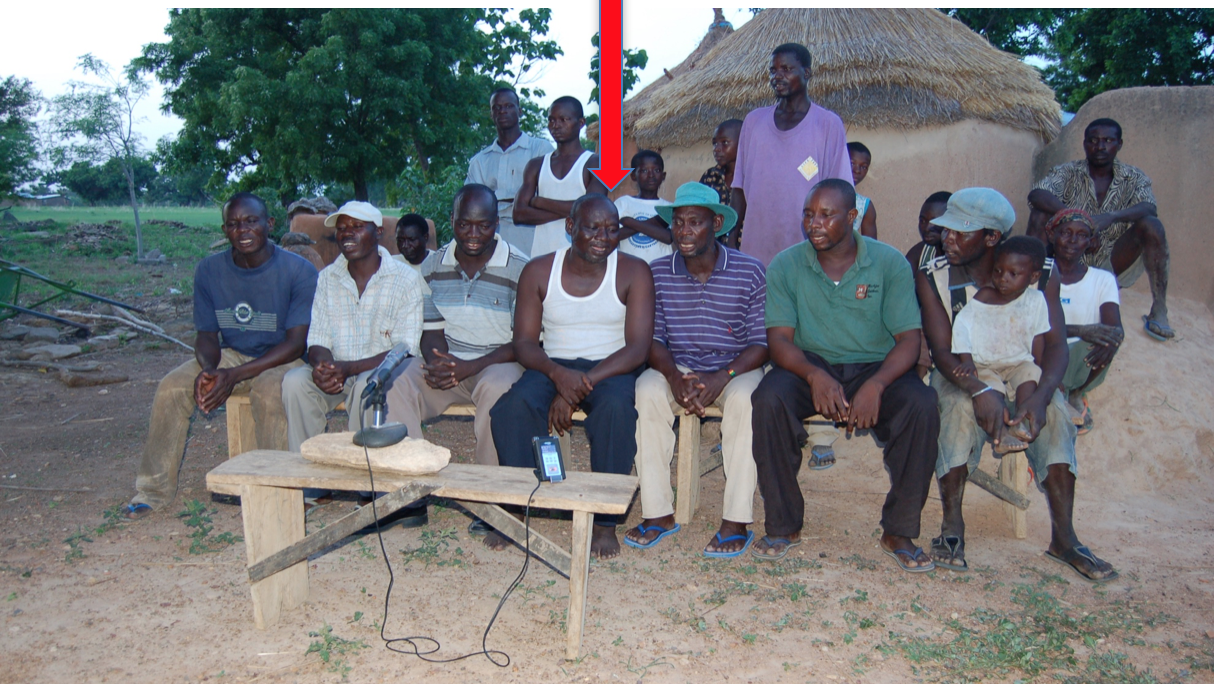
\includegraphics[scale=0.55]{../figures/apia.png}
\caption{Riddles and Folktale narration session at Yorogo near Bolga by Apia (middle in singlet and arrowed) supported by his team members in the front row left and right. Picture taken in July 2010.}

\end{figure}


\begin{figure}
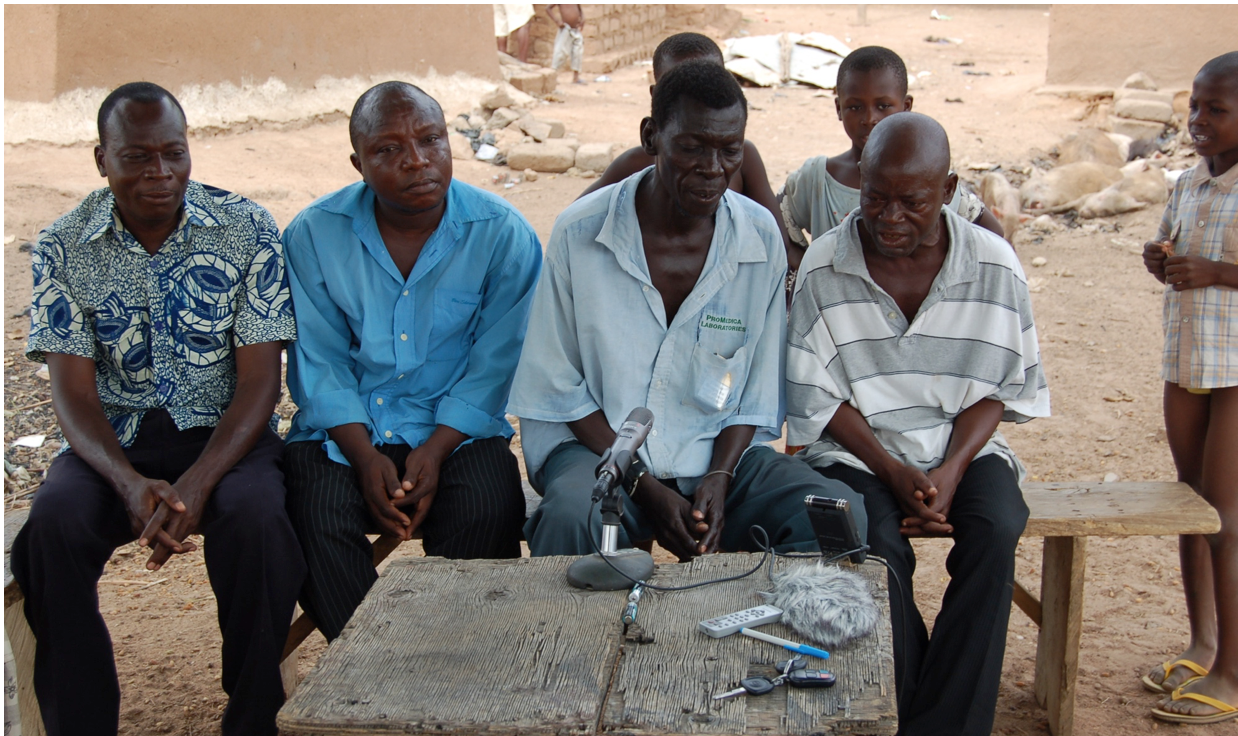
\includegraphics[scale=0.55]{../figures/adagesaana.png}
\caption{Adagesaana (extreme right) from Bolga Soe with his colleague Narrator Nsoh Atimbila from Bolga 
 	  Bukere (second from right) at a narration session. Extreme left is Philip Anangina who has been my 
 	key documentation team member in Bolga and his friend Mba (my former student) who
 	 accompanied us. Picture taken in April 2010.}

\end{figure}


\begin{figure}
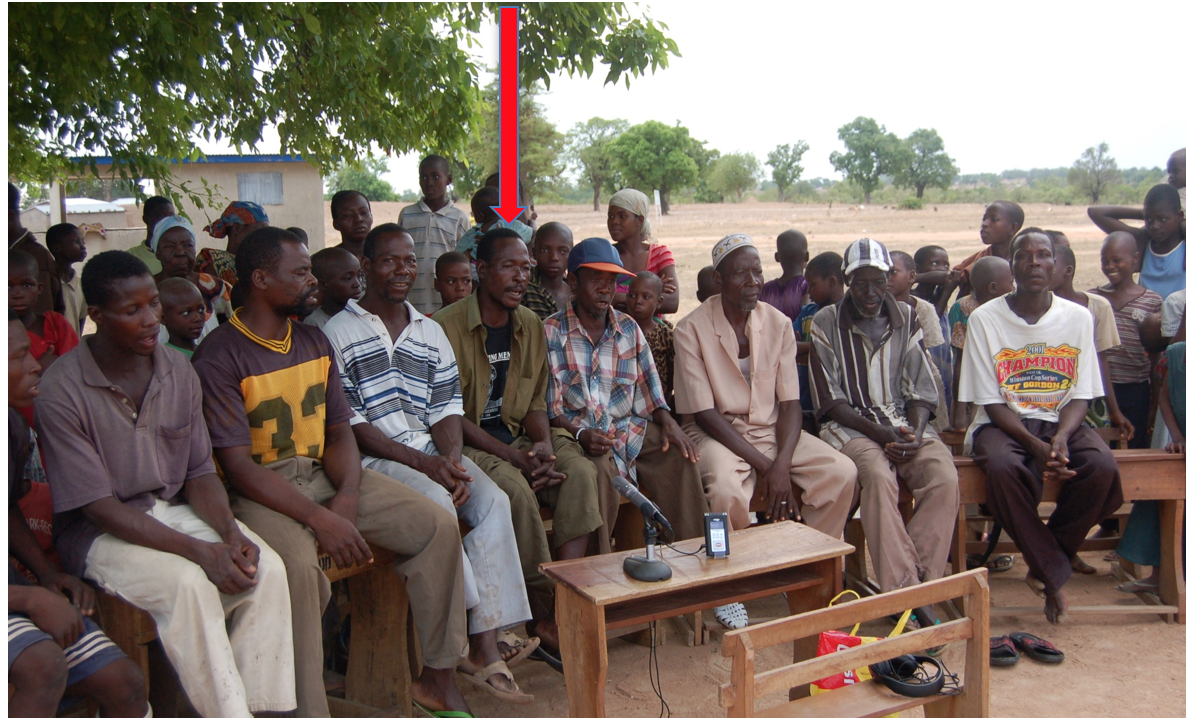
\includegraphics[scale=0.55]{../figures/abugebiire.png}
\caption{Sung Folktale performance session at Sapooro by Abugebiire (arrowed) and his team members. Picture taken in April 2010.
}

\end{figure}


\begin{figure}
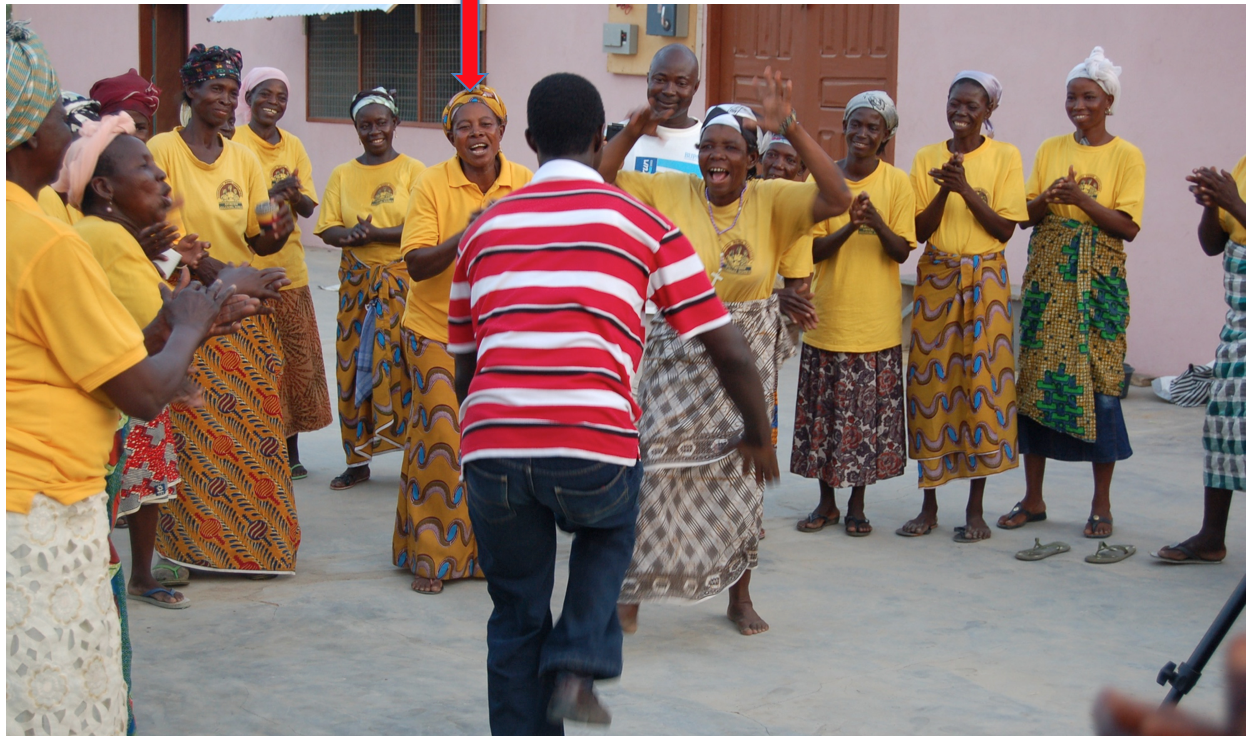
\includegraphics[scale=0.55]{../figures/sumbrongo.png}
\caption{Sumbrongo women performing women songs with the documenter (Samuel Atintono) dancing. Leader of the group (Nsoma, arrowed). Picture taken in April 2010.}
\end{figure}

\begin{figure}
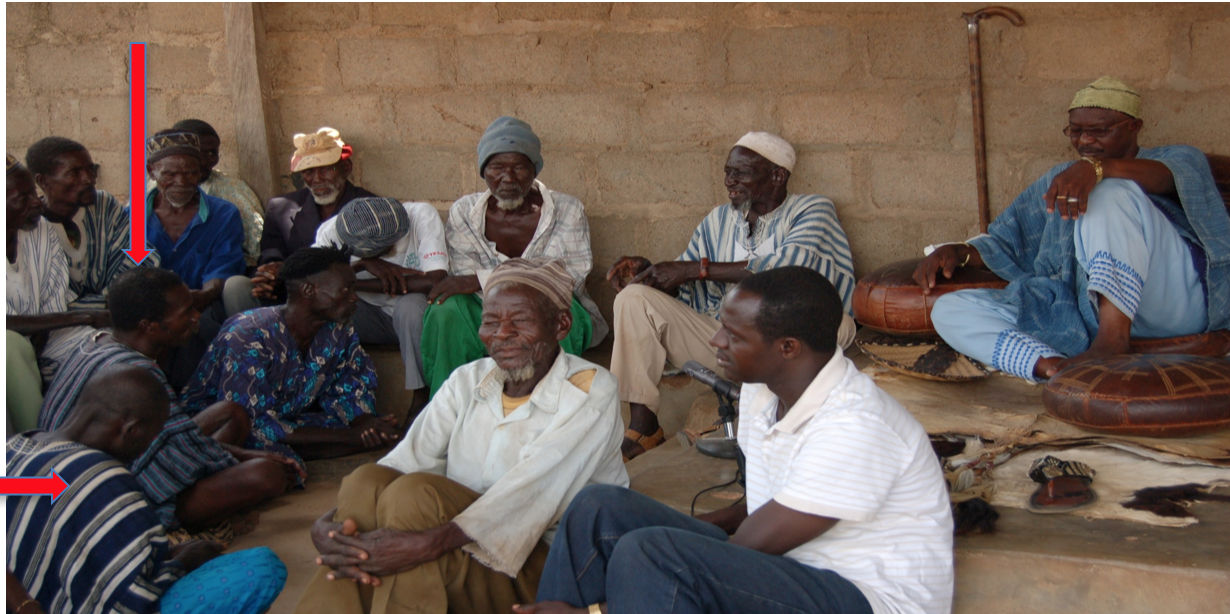
\includegraphics[scale=0.55]{../figures/bongo.png}
\caption{A traditional court trial on land dispute at the Bongo Chief’s Palace with the chief is seated 
 	on top right. The documenter, Samuel Atintono first from right in the first row. The arrowed are the 
 	two litigants. The rest are the chief elders (Picture taken in April 2010).}

\end{figure}


\section{Strategies for documenting the oral genres}

In this section, I discuss some of the strategies that were employed in documenting these genres. The first strategy involves consultations with the gate keepers in the community in order to gain access to both consultants and places for the documentation. They include chiefs, elders,  and some local political leaders,  in the case of Ghana, the Assembly member who represents the community at the district assembly. Being a native speaker or a member of the community does not necessarily grantee you easy access to people and places. I belong to the community but the fact that I had returned to document these genres meant I needed to obtain permission from the community leaders before I could start the project. The only advantage that I had as a native speaker was that the people were very receptive to me and in most cases I also knew the people to contact for particular information. 

There is also the issue of making clear the goals of the project by the fieldworker to enlist the support of the community. In this respect, you must build trust between you and the community members. They are only willing to cooperate in the execution of the project when they have trust and are convinced about the goals of the project. Some members complained that previous researchers who came to record some data never returned to the community. However, they later saw their materials in publications or even in documentaries shown on national TV without their consent.

The fieldworker must also demonstrate transparency about the end result of the documentation products. The community members needed to know where the recorded folktales would end up. Some members complained about previous researchers not allowing them to have access to the recordings that they have taken from them. In my case, I made them to understand that after the documentation they would be given some of the audio and video recordings and I did give them the DVDs after the project. It is important to give community members some of the products created out of the documentation such as DVDs of audio and video recordings, simple literacy materials, wordlists or dictionaries. This way, they will appreciate and support the project.

One other strategy that was adopted in the fieldwork was to involve the help and support of the local people who have high interest in the documentation and preservation of the language and cultural resources. The five people that I recruited were all self-motivated to participate in the project and this also helped me to record a lot of genres. They could go on their own to document some events without my presence. When you involve active community members in your documentation project they may have privileges to access some community events that the fieldworker will not be allowed to participate and record.  A typical example in my documentation was a situation where I wanted to document ritual genres associated with the burial rituals in Bolga and the pallbearers would not accept an uninitiated person to observe the rituals. Fortunately, one of my documentation team members had been initiated as a pallbearer so he had the privilege of participating and recording the rituals and also interviewing the expert pallbearers.

The promotion of the documentation project on local radio or TV stations in the community where it is possible can also help to whip up the community interest in the project. It will also create the opportunity among the community members to become aware of the project goals so that they can support it. It will be helpful to let the local team members do the talking about the need for the documentation project. I had a weekly programme of about 45 minutes to discuss my documentation project on a local radio station called Gurenɛ Style in Bolga which ran its programmes using only Gurenɛ. The response from the community members was very impressive as it made people to discuss why families should speak to their children in Gurenɛ and suggested ways to revitalise and preserve the folktales.  This proved to be very helpful as those who listened to the programme expressed their appreciation for the initiative and also pointed out to me some other experts knowledgeable in some of the genres for further contact. 

Another crucial thing that I did was to play some of the folktales that I have transcribed on the radio stations and it generated a lot of interest. People were surprised to hear these dying genres being played on the radio. I left a lot of the audio recordings of the songs and the folktales with the radio station to play during our programme time after we had left. Other radio stations soon learnt about them and also collected them to play at their stations. The outcome of this, is that many people became more interested in the use of these folktales.


\section{Challenges on the field}

As observed by \cite{Bowern2015} every fieldwork situation has its own unique problems. There were a number of challenges that I encountered during the fieldwork which affected the progress of my work. They range from consultant’s work schedules to equipment malfunctioning. I discuss each of these issues below.

Disappointments from my consultants with respect to meetings on time or postponement of meetings were a major factor. You may schedule a meeting at 1.00pm and they turn up at 2.00pm or later. In some instances, they may not even turn up. Some consultants are also very difficult to track for work. An example is one folktale narrator in Bolga that I had to follow him for six weeks before I was able to get him to start the narration of his tales. He would schedule an appointment for a meeting on a market day which comes every three days but whenever I met him he would give an excuse but will request that I buy him a local drink. He was a very slippery person but very knowledgeable in the riddles and folktale genre so I had no option but to continue to look for him on every Bolga market day to buy him the drinks until I finally had him in the sixth week to start the narration. 

As a fieldworker, one needs to be patient with consultants and also you must adjust to the activities and time of your consultants to succeed in your fieldwork. Some other consultants had emergencies and could not honour appointments.

One other challenge that I had was the observance of cultural norms and social practices in the communities. While on the field, I noticed that whenever there was a funeral in any of the communities that I work, there will be no work for a few days. Particularly, if the funeral affects the consultant’s family member or their neighbours you may be required to attend and express your condolences. You will also be required to make a small donation of cash or provide a local drink. The period of my documentation coincided with the performance of funerals in the communities and I frequently encountered these situations which made me to postpone scheduled appointments. 

I have had invitations very often from my consultants to attend other social events such as weddings, birthday or anniversary celebrations of churches or prominent community members. The fieldworker’s physical presence is often very much appreciated and an expectation of making a donation in cash or kind. This could be time consuming and some cost involved. Even though these events do not directly relate to our documentation project but they help to maintain a good working relationship with the community. It is also important to observe these cultural norms and practices in the community to avoid potential breaking of these norms.  

One other social event that was also a bit disruptive was friends’ invitation to socialising events such as drink sessions at local pubs. I found myself busy doing some work on my documentation data and hardly had time to attend them but to my friends, I must honour them otherwise I will be labelled as showing off.  This requires some negotiations to attend some and leave others else it will derail your work plan.

In the documentation literature, a lot has been said about how to record events and the type of equipment to take to the field for optimum results \citep{Bowern2015, Woodbury2003, AustinGrenoble2007}.  It is important to be aware of the type of event that you can record and also the type of equipment that is appropriate to use. Recording of some cultural performances such as the traditional war dances which involved the performers running on the field as in Figure 7 below was very difficult to position the camera in a good angle to record because of the fast movement.  

\begin{figure}
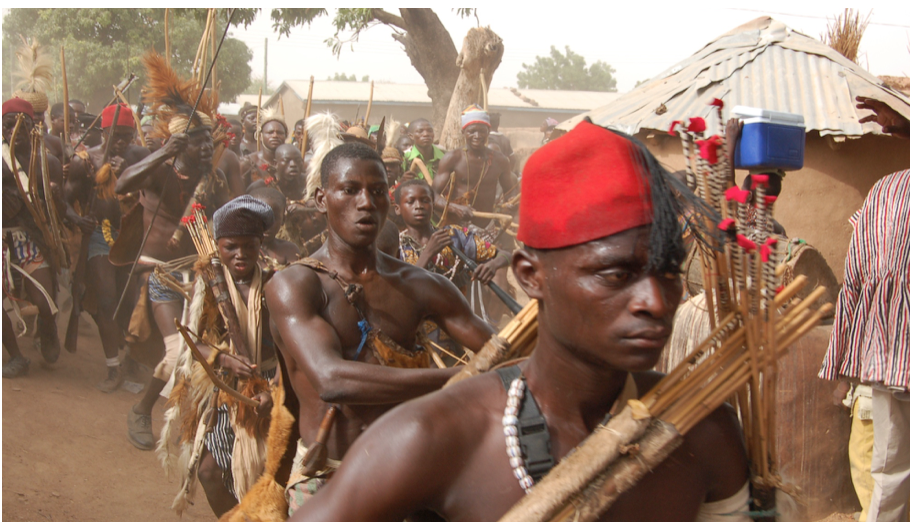
\includegraphics[scale=0.55]{../figures/bolga_soe.png}
\caption{A group of war dancers (the leader is in front) from Bolga Soe at a funeral. Picture taken in May 2010}
\end{figure}


Also, the dancers sang along while performing the dance and this created an excessive noise coupled with the noise made by the enthusiastic crowd who follow them. Thus, running to catch pace with them and record made the images to be unstable. The only time we had good images of the war dancers was when they performed at the front of the compound in a circular movement. Further, we have had instances where some of the audience deliberately shout or pass through the path of the camera lens just to be captured in the video.

Another crucial issue to note while on the field is to ensure that the recording equipment is constantly in good condition for an efficient workflow while on the field (cf. \citealt{Bowern2015}). Even though you might have charged your batteries and tested them the previous night before going to the field it is important to frequently monitor the equipment because the weather conditions can affect its performance. Our audio recorder with soft plastic case easily melted under the heat of the tropical sun and this sometimes led to the malfunctioning of the recorder. In northern Ghana, between April and June the weather usually gets hotter peaking between 30--40 degrees celsius. Thus, the audio recorders with metal or hard plastic casing are much better under such conditions.

One other important issue a fieldworker should consider is how to manage efficient power supply to the recording equipment during fieldwork. In some of the communities that I worked there was no electricity and in others there was electricity but it was very unstable and could go on and off for every 30 minutes. I used lithium and alkaline rechargeable batteries for the audio recorder. But we have had instances where the batteries depleted completely even though they were fully charged. You need to have sufficient rechargeable batteries for the digital audio and camcorders. You must remember to charge them over night. I found out that Lithium batteries were far better than Alkaline. In the tropics, heat can cause the batteries to discharge faster.

\begin{figure}
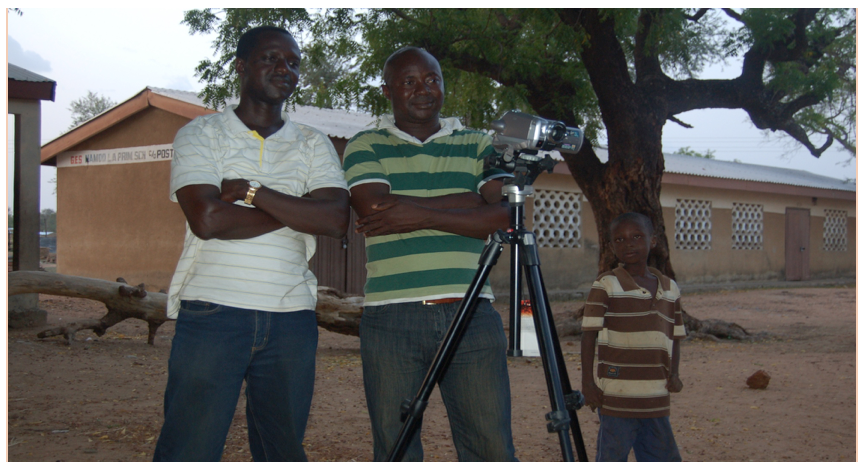
\includegraphics[scale=0.55]{../figures/samuel.png}
\caption{Samuel Atintono (left, documenter) and James Akolgo (Right) monitoring the video 
 		camera during a folktale narration session at Namoo, Bongo. Picture taken in May 2010.}

\end{figure}


As you can see in Figure 8, the documenter and his team member are monitoring the battery level of the camera and to ensure that it was actually recording the event. It is  important to ensure that you do not lose your recording as a result of the battery or the camera not working. 


\section{Conclusion}
The paper discussed my personal experience of documenting Gurenɛ oral genres in northern Ghana and notes its significant contribution in saving the disappearing genres such as riddles and folktales, sung folktales and songs. It is noted that though Gurenɛ may not be classified as an endangered language because of the existence of a large number of speakers and intergenerational transmission some aspects of its linguistic resources which include riddles and folktales are vanishing as there are only a few elderly people living today who have expertise in them and they die along with their knowledge.

The Gurenɛ documentary corpus contains many hours of both audio and video recordings of different types of oral genres e.g, riddles, folktales, songs, ritual texts, traditional court proceedings, descriptive texts and cultural performances. Most of these data have been transcribed, annotated and archived. 

The paper also outlined a number of strategies that are required in order to be able to undertake a successful fieldwork which include community entry protocols, building trust among community members, ensuring transparency of the project, community members’ participation in the project, advocacy and rewarding them with the documentary products. Some challenges on the field that can significantly affect the progress of work on the field have also been discussed. They include delays in consultant’s work schedules, the observance of cultural norms in the community, participation in social events, managing recording and equipment to ensure efficient workflow.


%\section*{Abbreviations}
%\section*{Acknowledgements}
 

\printbibliography[heading=subbibliography,notkeyword=this]

\end{document}
